\documentclass{article}
\usepackage[utf8]{inputenc}
\usepackage{typearea}
\usepackage{multirow}
\usepackage{color, colortbl}
\usepackage{caption}
\usepackage{subcaption}
\usepackage{graphicx}
\usepackage{float}
\usepackage{lipsum}
\usepackage[pdftex]{hyperref}
\definecolor{Gray}{RGB}{231, 230, 230}

\title{Exercício 2 - Métodos dos Gradientes Conjugados}
\author{Lorena B. Bassani}
\date{2021}

\begin{document}

\maketitle

\begin{abstract}
    Este documento relata os resultados do segundo exercício da disciplina de Algoritmos Numéricos II, no semestre 2021/01 EARTE. Observar o comportamento do Método dos Gradientes Conjugados para um conjunto de matrizes esparsas da \textit{SuiteSparse Matrix Collection}\footnote{\href{https://sparse.tamu.edu}{https://sparse.tamu.edu}}.
\end{abstract}

\section{Introdução}
Para este exercício, foram utilizadas sete matrizes quadradas esparsas, a \textit{mesh3em5} de $289$ linhas e colunas, \textit{plat362} com $362$ linhas, a \textit{662\_bus} com $662$, \textit{s1rmq4m1} com $5.489$, a \textit{pdb1HYS} com $36.417$ e a \textit{Dubcova3} de dimensão $146.689$, obtidas da coleção de matrizes esparsas \textit{SuiteSparse Matrix Collection}. Nessas sete matrizes, foram realizadas análises quanto ao comportamento do métodos dos gradientes conjugados, utilizando a ferramenta Octave. Na seção~\ref{sec:resultados} são relatadas algumas observações sobre a utilização deste método para resolução de sistemas lineares, e na última parte do trabalho, nas seções~\ref{sec:figures} e~\ref{sec:tabelas}, se encontram as figuras e as tabelas com os resultados obtidos, respectivamente.

\section{Exercício Proposto -- Método dos Gradientes Conjugados}
\label{sec:resultados}
O objetivo deste exercício é observar o comportamento de matrizes esparsas na solução de sistemas lineares via método dos gradientes conjugados, que é um método iterativo não estacionário. Para isto, as matrizes escolhidas foram utilizadas como matriz de coeficientes para solução de sistemas lineares através de método nativo do Octave, e foram observados uma série de fatores quanto ao comportamento das matrizes a respeito da convergência da resposta e seu número de condicionamento.

O método dos gradientes conjugados é um dos métodos que levariam a uma resposta exata em $n$ passos, a menos de erros de arredondamento, porém, levando em consideração que a maior parte do decrescimento do erro ocorre nos passos primários, ele é tratado como método iterativo, parando após atingir critérios de tolerância do erro. Isso faz com que o método, para matrizes bem condicionadas, convirja rapidamente, em pouquíssimas iterações quando comparado a dimensão da própria matriz. Essa é sua grande vantagem sobre os métodos dos gradientes puro, pois, caso comece a chegar a um alto número de iterações, pelo fato de realizar mais operações custosas que este, ele se tornaria menos interessante.

Sistemas mal condicionados amplificam erros de arredondamento, geralmente pela grande diferença entre a magnitude dos autovalores desta, apresentando convergência lenta ou nenhuma. Este caso pode ser observado nas matrizes que não convergiram ao final da aplicação do método (apresentam \textit{flag} 1), como a \textit{pdb1HYS} de acordo com as tabelas~\ref{tab:resultados-5k-6} e \ref{tab:resultados-5k-11}. Em especial, nesta última, a matriz \textit{s1rmq4m1} não convergiu, mesmo levando um número muito próximo de $n$ iterações. De fato, na tabela \ref{tab:resultados-10k-11} vemos que, para tolerância $10^{-11}$ tanto a \textit{s1rmq4m1} quanto a \textit{662\_bus} e \textit{plat362} levam mais que $n$ iterações para atingirem o critério de tolerância, e seus gráficos mostram claramente, enquanto a \textit{bcsstk36} nem mesmo converge e a \textit{pdb1HYS} para por estagnação do erro (\textit{flag} 3). Quando visualizando os gráficos dos resíduos em cada iteração, é possível ver o erro aumentar e diminuir quase que aleatoriamente, comportamento que indica que o método começa a caminhar para distanciamento da resposta real ao invés de ficar mais próximo. Observando os números de condicionamento que foram possíveis calcular\footnote{As matrizes \textit{pdb1HYS} e \textit{Dubcova3} não permitiram o calculo do número de condicionamento por serem muito grandes, causando fechamento forçado do programa Octave depois de certo tempo do início da operação. A operação de cálculo de condicionamento é tão ou até mais custosa do que a própria solução do sistema linear, podendo até não ser possível em alguns casos, como observado.}, todas são matrizes mal condicionadas, com números de condicionamento maiores que $10^5$, muito maior que 1.

Apesar disso, apenas as matrizes \textit{plat362} e \textit{bcsstk36} retornaram com norma do máximo da solução muito acima do valor esperado, que seria 1. Isso significa que, de certa forma, apenas essas duas matrizes retornaram com ao menos alguma posição fora do valor da solução exata por um erro muito grande, mesmo que tenham convergido em certas ocasiões. Todas as outras conseguiram, mesmo que contando com a sorte, encontrar uma resposta satisfatória no final.

As matrizes \textit{mesh3em5} e \textit{Dubcova3} mostraram um comportamento muito satisfatório em todas as situações em que foram submetidas ao método, convergindo com um número muito inferior de interações quando comparado as suas dimensões. A matriz \textit{mesh3em5} não apenas possui um número de condicionamento baixo, 4,966, como também é diagonal dominante, sendo uma matriz extremamente vantajosa para aplicação do método. É possível ver em seus gráficos que ambas matrizes apresentaram comportamento de queda linear na dimensão do erro, levando a convergência extremamente rápida do método, com poucas ou nenhuma subida do valor do resíduo durante todo o processo. Com isso, é possível declarar que sejam matrizes bem condicionadas, e que elas demonstram todas as vantagens da aplicação deste método quanto a rapidez da convergência e quantidade mínima de iterações que utiliza para chegar a um resultado satisfatório.

\storeareas\normalsetting
\KOMAoption{paper}{landscape}
\areaset{2\textwidth}{.95\textheight}
\recalctypearea

\section{Figuras dos resultados observados}
\label{sec:figures}

\begin{figure}[H]
    \centering
         \centering
         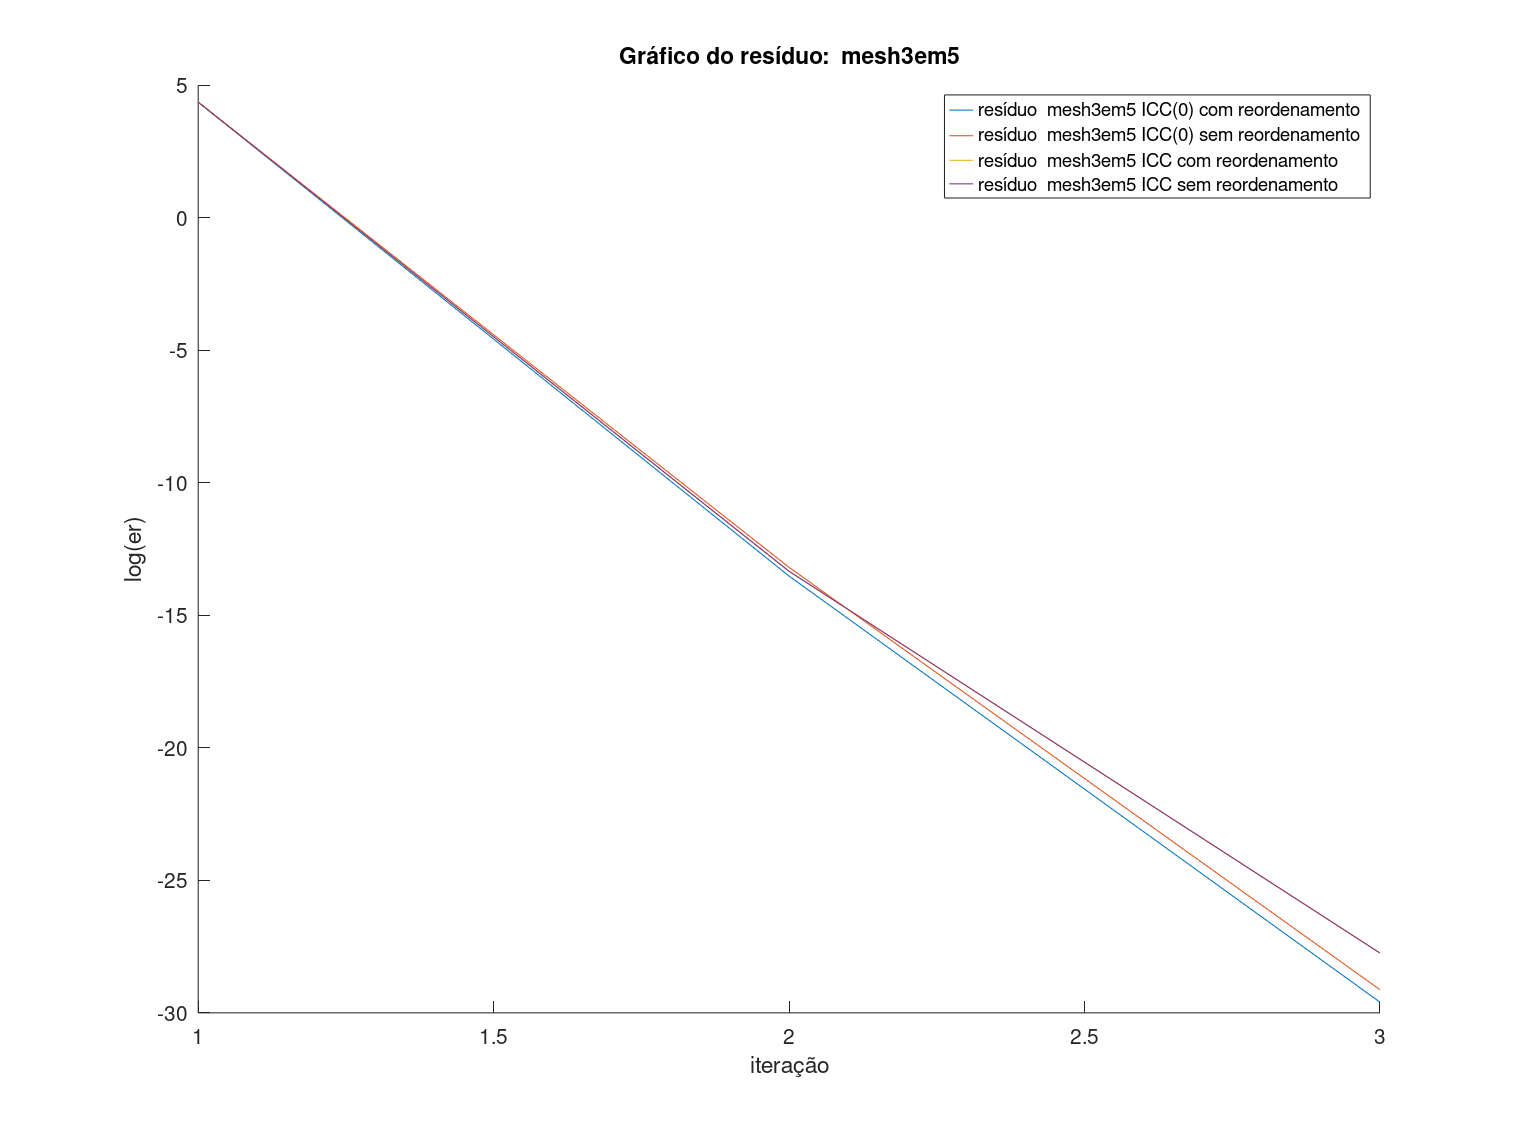
\includegraphics[width=.6\linewidth]{images/mesh3em5.png}
         \caption{Gráfico do Resíduo da matriz \textit{mesh3em5}}
         \label{fig:mesh-res}
\end{figure}

\begin{figure}[H]
    \centering
         \centering
         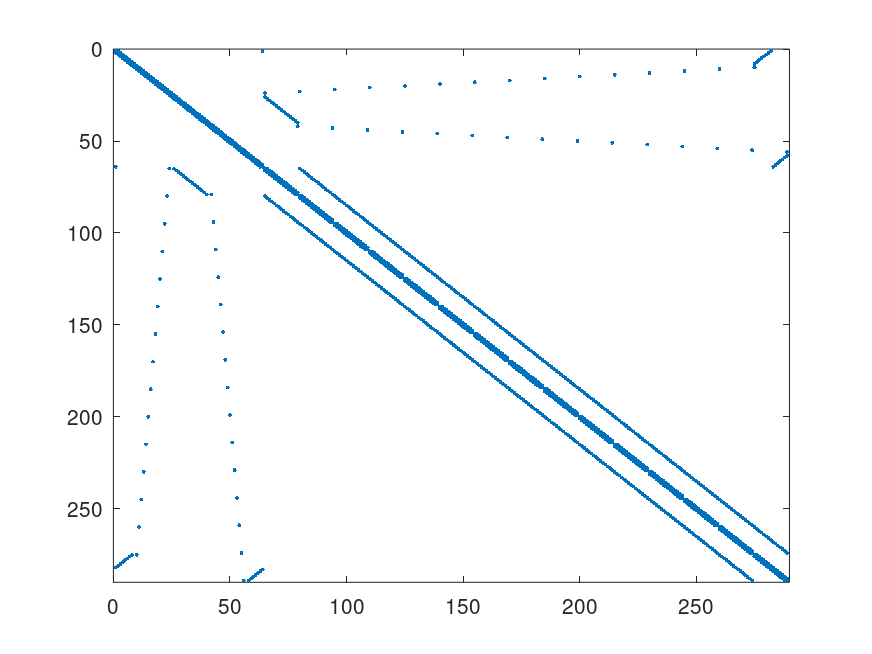
\includegraphics[width=.5\linewidth]{images/mesh3em5_spyA.png}
         \caption{Spy de da matriz \textit{mesh3em5}}
         \label{fig:mesh-spy-a}
\end{figure}

\begin{figure}[H]
    \centering
    \begin{subfigure}[t]{0.4\linewidth}
         \centering
         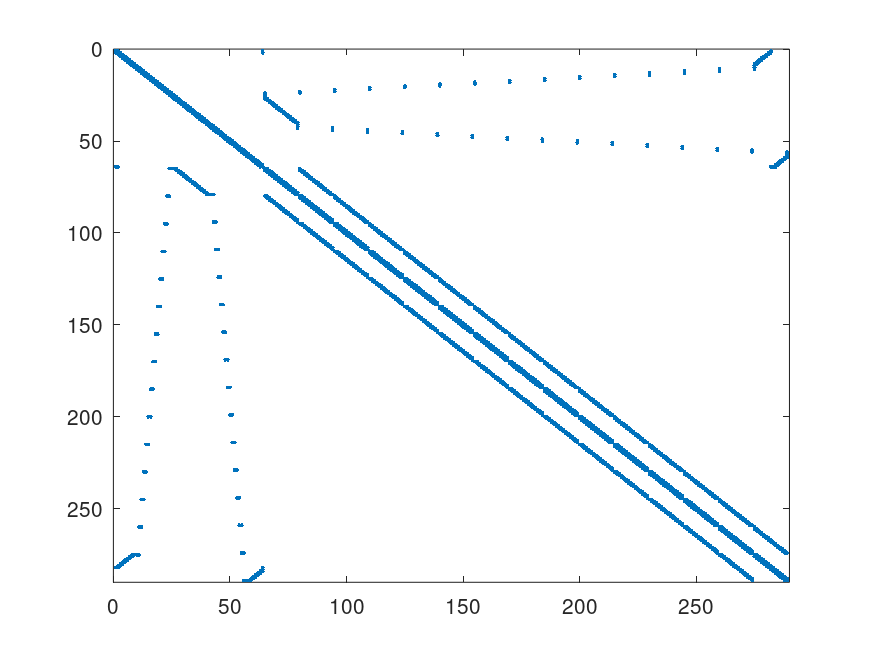
\includegraphics[width=\textwidth]{images/mesh3em5_spyM_ICC(0)_sem.png}
         \caption{Spy após ICC(0) sem reordenamento}
         \label{fig:mesh-icc0-sem}
    \end{subfigure}
    \quad
    \begin{subfigure}[t]{0.4\linewidth}
         \centering
         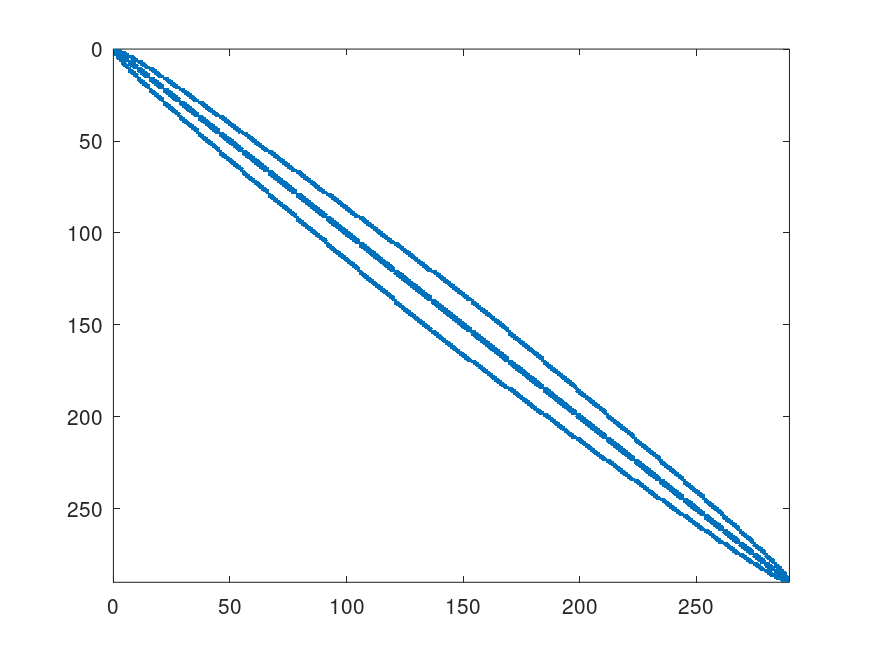
\includegraphics[width=\textwidth]{images/mesh3em5_spyM_ICC(0)_com.png}
         \caption{Spy após ICC(0) com reordenamento}
         \label{fig:mesh-icc0-com}
    \end{subfigure}
    \par\bigskip
    \begin{subfigure}[t]{0.4\linewidth}
         \centering
         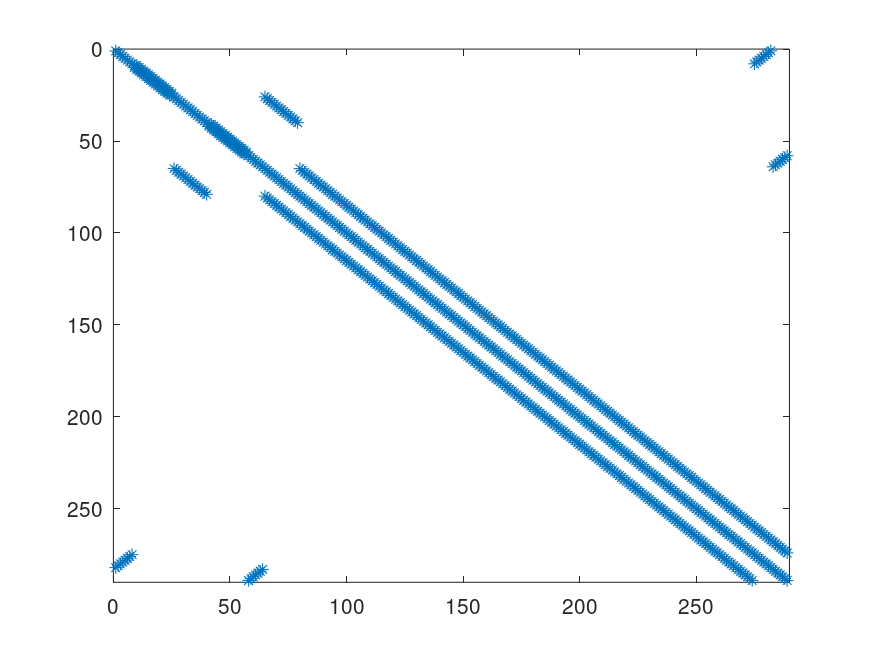
\includegraphics[width=\textwidth]{images/mesh3em5_spyM_ICC_sem.png}
         \caption{Spy após ICC sem reordenamento}
         \label{fig:mesh-icc-s}
    \end{subfigure}
    \quad
    \begin{subfigure}[t]{0.4\linewidth}
         \centering
         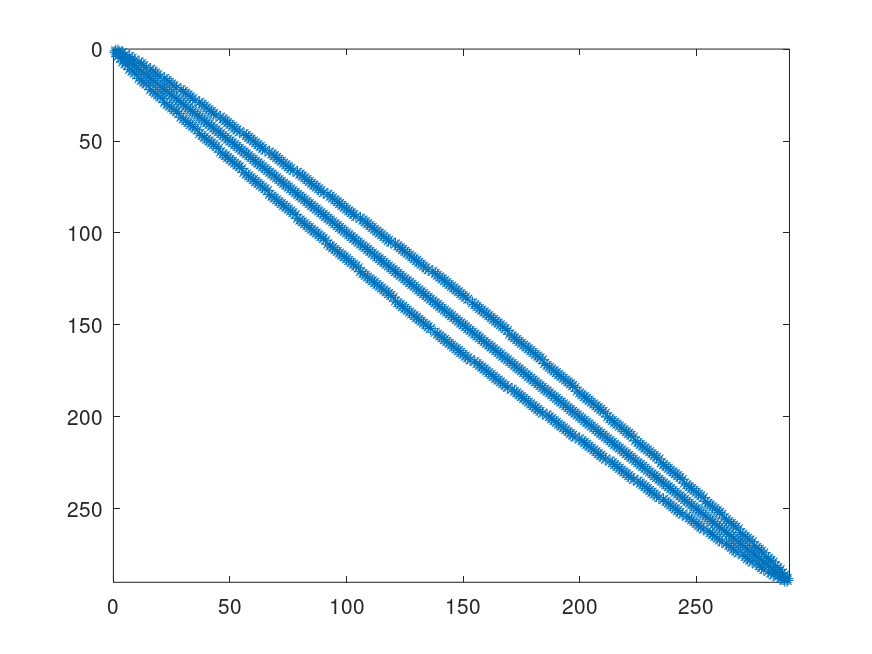
\includegraphics[width=\textwidth]{images/mesh3em5_spyM_ICC_com.png}
         \caption{Spy após ICC com reordenamento}
         \label{fig:mesh-icc-c}
    \end{subfigure}
    \caption{Gráficos do preenchimento de \textit{mesh3em5}.}
    \label{fig:mesh}
\end{figure}
\begin{figure}[H]
    \centering
    \begin{subfigure}[t]{0.4\linewidth}
         \centering
         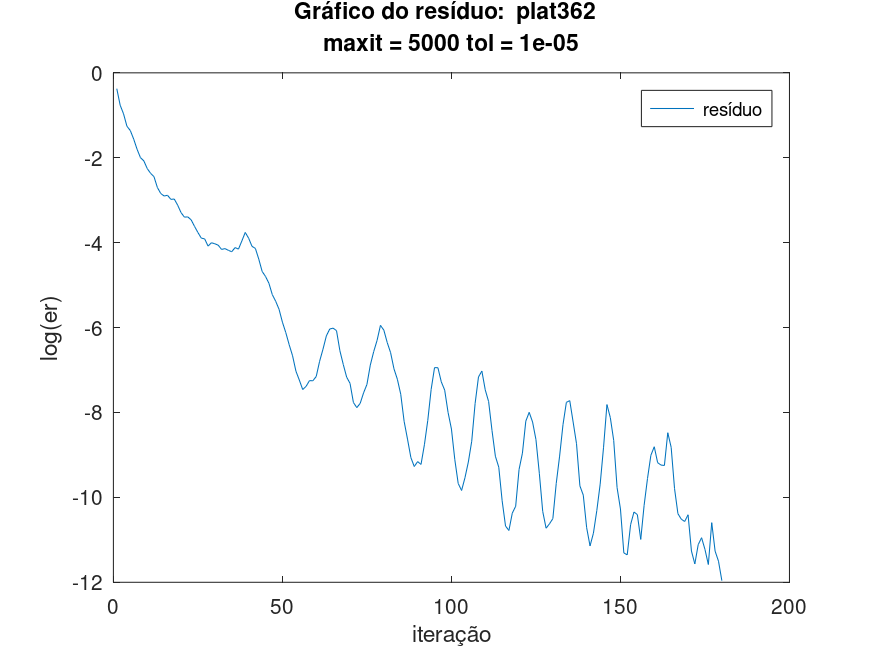
\includegraphics[width=\textwidth]{image/plat362_5000_-6.png}
         \caption{Gráfico do Resíduo para maxit $= 5.000$ e tol $=10^{-6}$}
         \label{fig:plat362-5-6}
    \end{subfigure}
    \quad
    \begin{subfigure}[t]{0.4\linewidth}
         \centering
         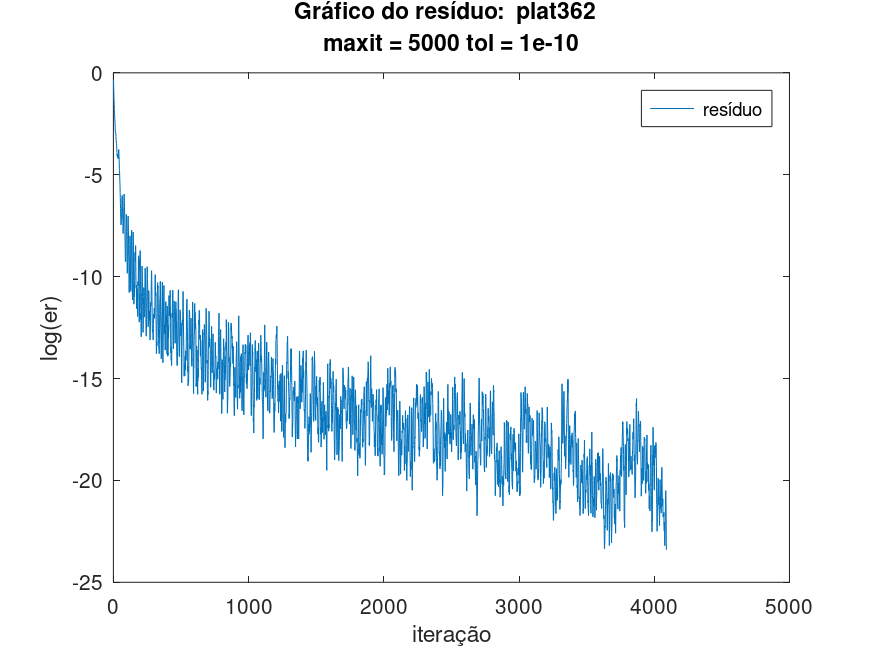
\includegraphics[width=\textwidth]{image/plat362_5000_-11.png}
         \caption{Gráfico do Resíduo para maxit $= 5.000$ e tol $=10^{-11}$}
         \label{fig:plat362-5-11}
    \end{subfigure}
    \par\bigskip
    \begin{subfigure}[t]{0.4\linewidth}
         \centering
         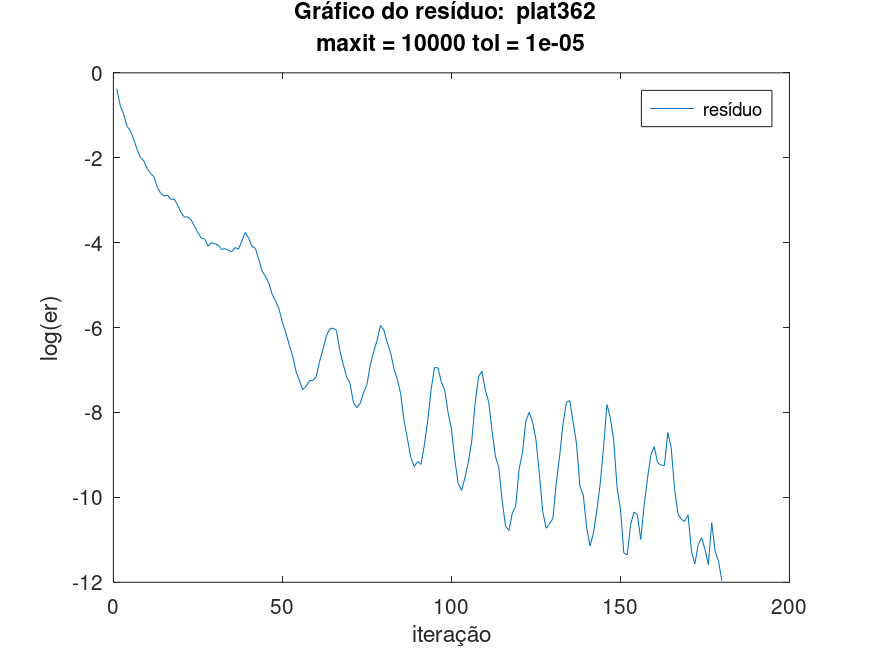
\includegraphics[width=\textwidth]{image/plat362_10000_-6.png}
         \caption{Gráfico do Resíduo para maxit $= 10.000$ e tol $=10^{-6}$}
         \label{fig:plat362-10-6}
    \end{subfigure}
    \quad
    \begin{subfigure}[t]{0.4\linewidth}
         \centering
         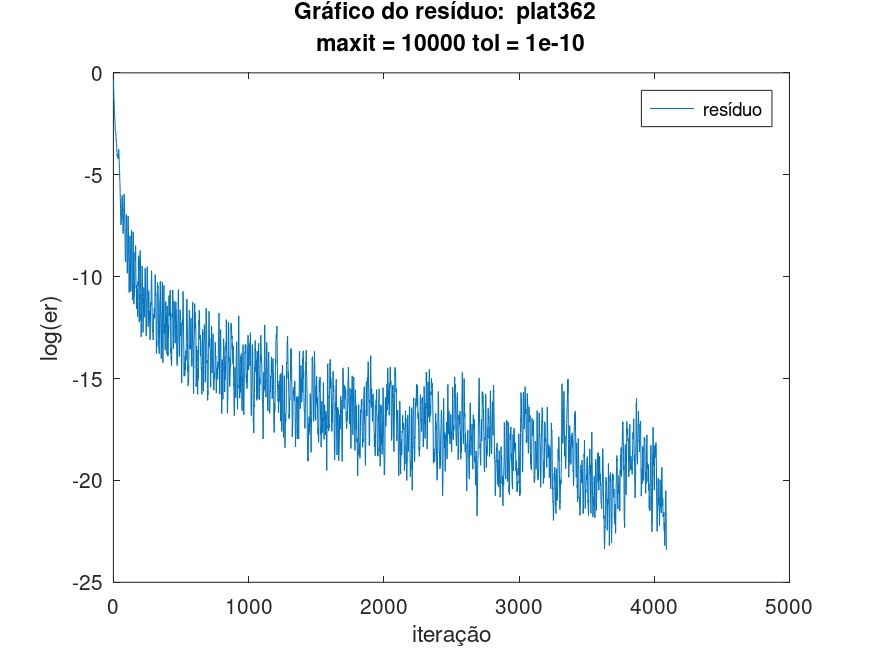
\includegraphics[width=\textwidth]{image/plat362_10000_-11.png}
         \caption{Gráfico do Resíduo para maxit $= 10.000$ e tol $=10^{-11}$}
         \label{fig:plat362-10-11}
    \end{subfigure}
    \caption{Gráficos dos resíduos para \textit{plat362}.}
    \label{fig:plat362}
\end{figure}
\begin{figure}[H]
    \centering
         \centering
         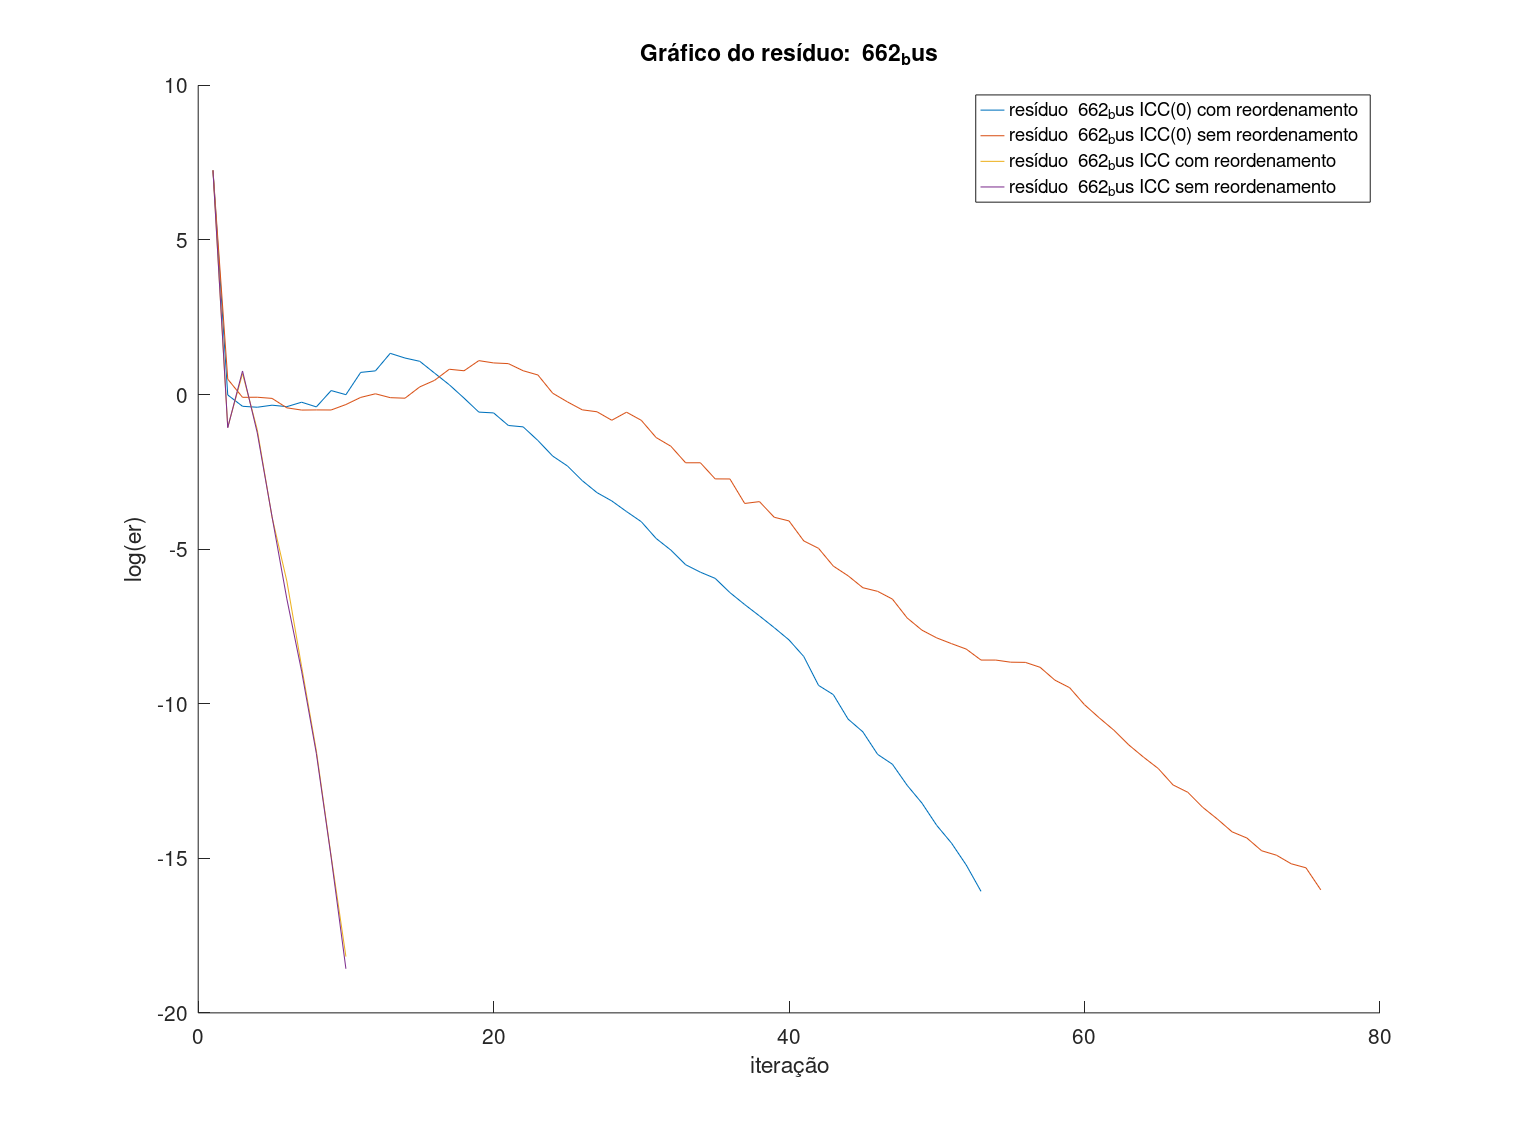
\includegraphics[width=.6\linewidth]{images/662_bus.png}
         \caption{Gráfico do Resíduo da matriz \textit{662\_bus}}
         \label{fig:bus-res}
\end{figure}

\begin{figure}[H]
    \centering
         \centering
         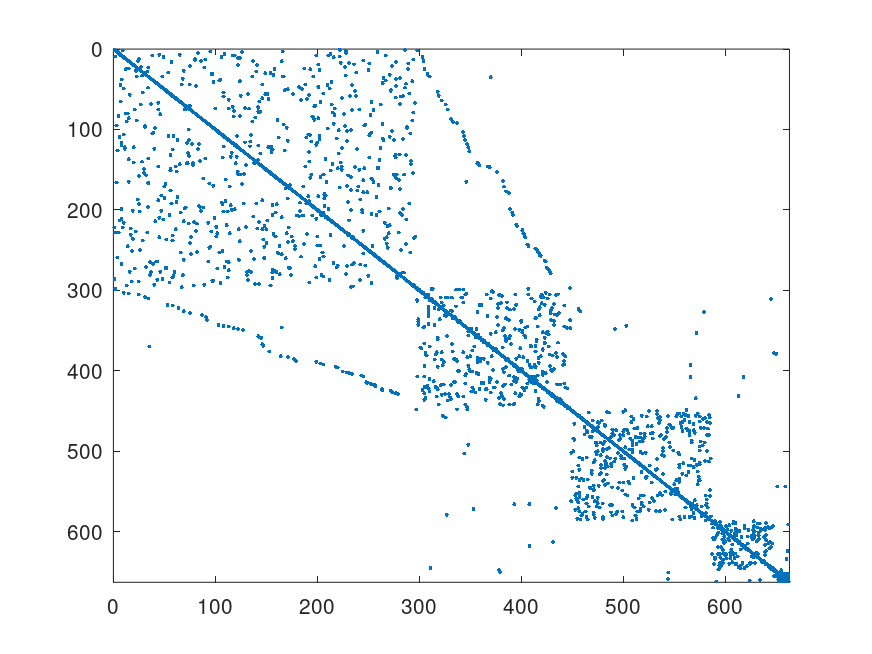
\includegraphics[width=.5\linewidth]{images/662_bus_spyA.png}
         \caption{Spy de da matriz \textit{662\_bus}}
         \label{fig:bus-spy-a}
\end{figure}

\begin{figure}[H]
    \centering
    \begin{subfigure}[t]{0.4\linewidth}
         \centering
         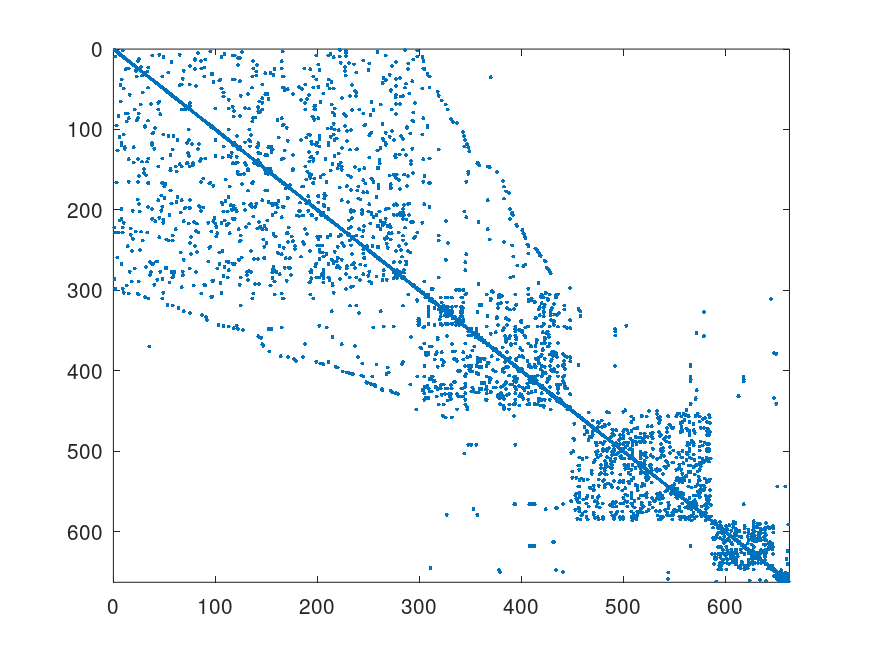
\includegraphics[width=\textwidth]{images/662_bus_spyM_ICC(0)_sem.png}
         \caption{Spy após ICC(0) sem reordenamento}
         \label{fig:bus-icc0-sem}
    \end{subfigure}
    \quad
    \begin{subfigure}[t]{0.4\linewidth}
         \centering
         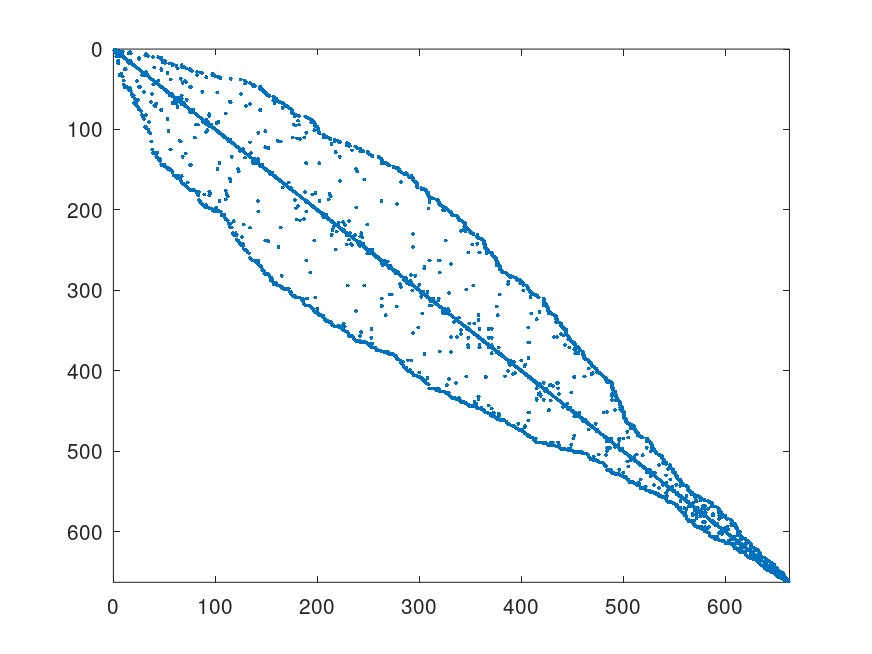
\includegraphics[width=\textwidth]{images/662_bus_spyM_ICC(0)_com.png}
         \caption{Spy após ICC(0) com reordenamento}
         \label{fig:bus-icc0-com}
    \end{subfigure}
    \par\bigskip
    \begin{subfigure}[t]{0.4\linewidth}
         \centering
         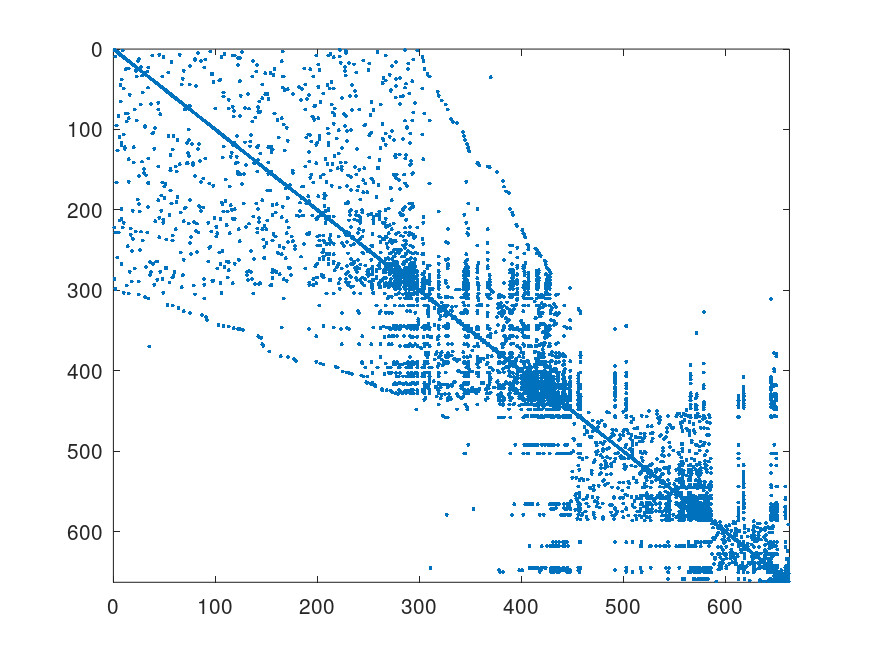
\includegraphics[width=\textwidth]{images/662_bus_spyM_ICC_sem.png}
         \caption{Spy após ICC sem reordenamento}
         \label{fig:bus-icc-s}
    \end{subfigure}
    \quad
    \begin{subfigure}[t]{0.4\linewidth}
         \centering
         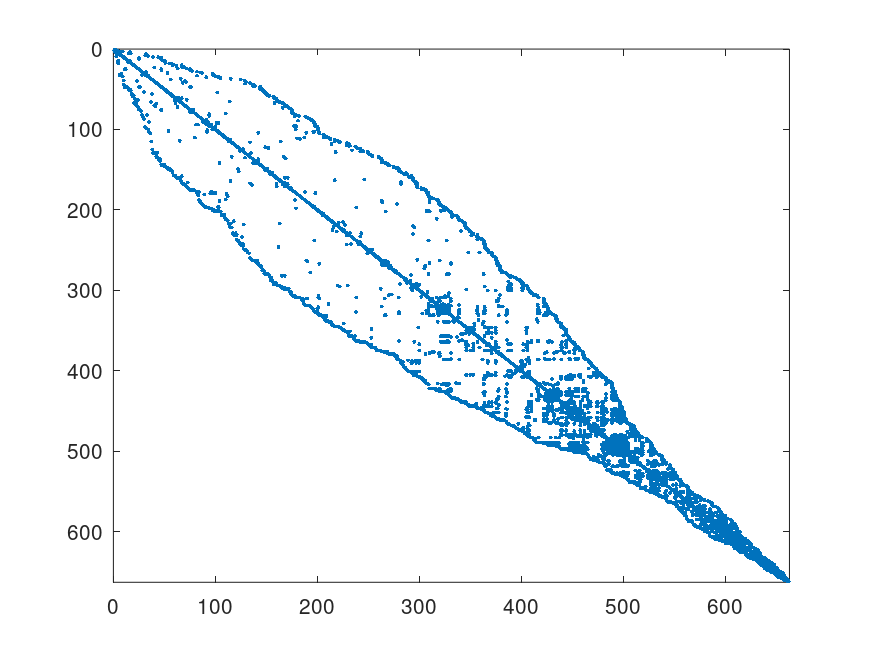
\includegraphics[width=\textwidth]{images/662_bus_spyM_ICC_com.png}
         \caption{Spy após ICC com reordenamento}
         \label{fig:bus-icc-c}
    \end{subfigure}
    \caption{Gráficos do preenchimento de \textit{662\_bus}.}
    \label{fig:bus}
\end{figure}
\begin{figure}[H]
    \centering
    \begin{subfigure}[t]{0.4\linewidth}
         \centering
         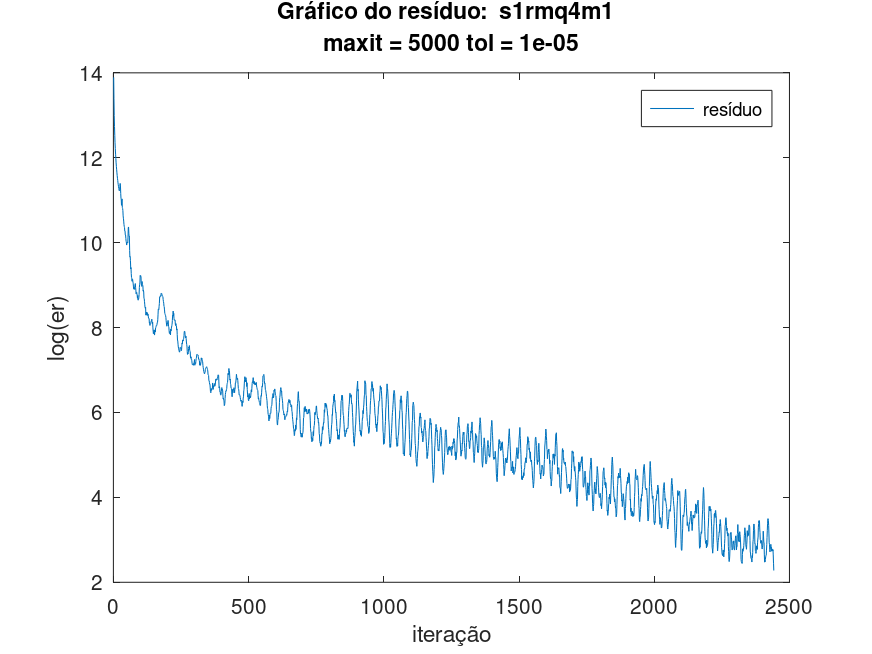
\includegraphics[width=\textwidth]{image/s1rmq4m1_5000_-6.png}
         \caption{Gráfico do Resíduo para maxit $= 5.000$ e tol $=10^{-6}$}
         \label{fig:s1rmq4m1-5-6}
    \end{subfigure}
    \quad
    \begin{subfigure}[t]{0.4\linewidth}
         \centering
         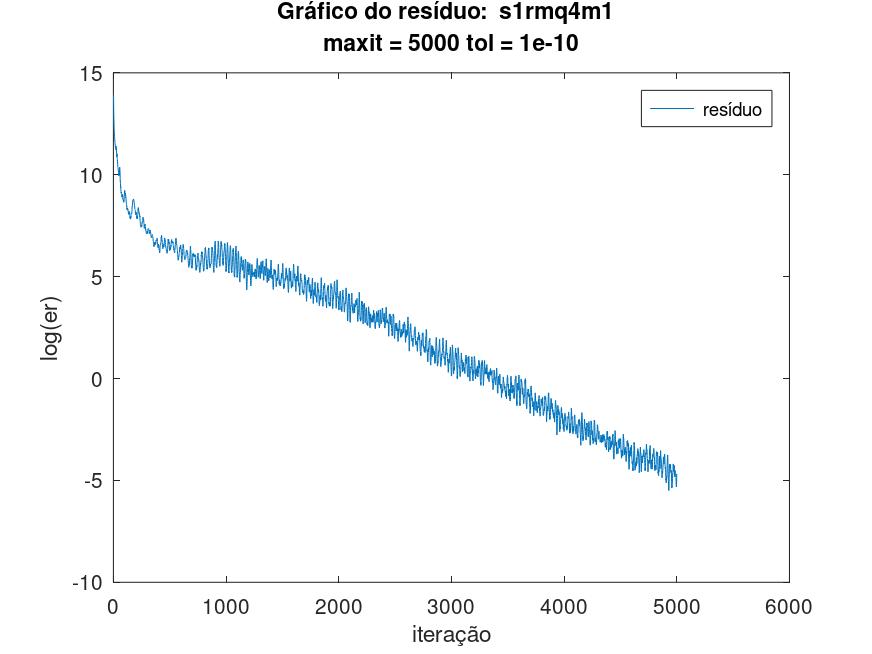
\includegraphics[width=\textwidth]{image/s1rmq4m1_5000_-11.png}
         \caption{Gráfico do Resíduo para maxit $= 5.000$ e tol $=10^{-11}$}
         \label{fig:s1rmq4m1-5-11}
    \end{subfigure}
    \par\bigskip
    \begin{subfigure}[t]{0.4\linewidth}
         \centering
         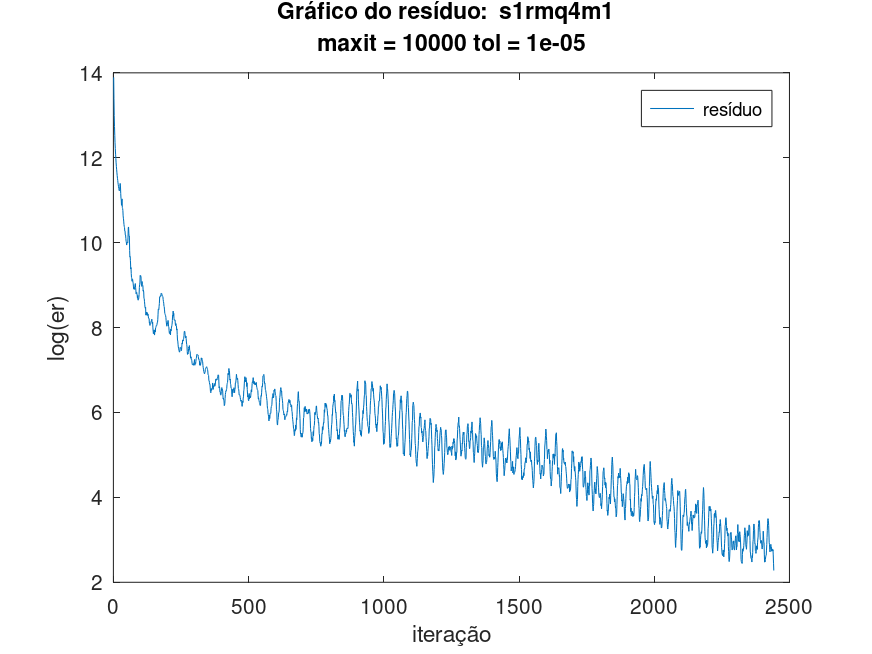
\includegraphics[width=\textwidth]{image/s1rmq4m1_10000_-6.png}
         \caption{Gráfico do Resíduo para maxit $= 10.000$ e tol $=10^{-6}$}
         \label{fig:s1rmq4m1-10-6}
    \end{subfigure}
    \quad
    \begin{subfigure}[t]{0.4\linewidth}
         \centering
         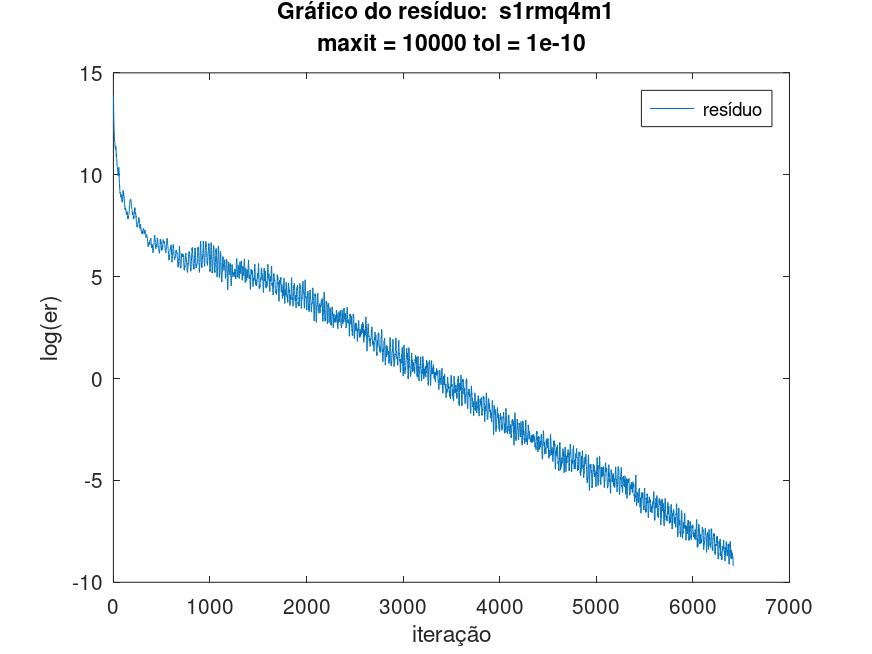
\includegraphics[width=\textwidth]{image/s1rmq4m1_10000_-11.png}
         \caption{Gráfico do Resíduo para maxit $= 10.000$ e tol $=10^{-11}$}
         \label{fig:s1rmq4m1-10-11}
    \end{subfigure}
    \caption{Gráficos dos resíduos para \textit{s1rmq4m1}.}
    \label{fig:s1rmq4m1}
\end{figure}
\begin{figure}[H]
    \centering
    \begin{subfigure}[t]{0.4\linewidth}
         \centering
         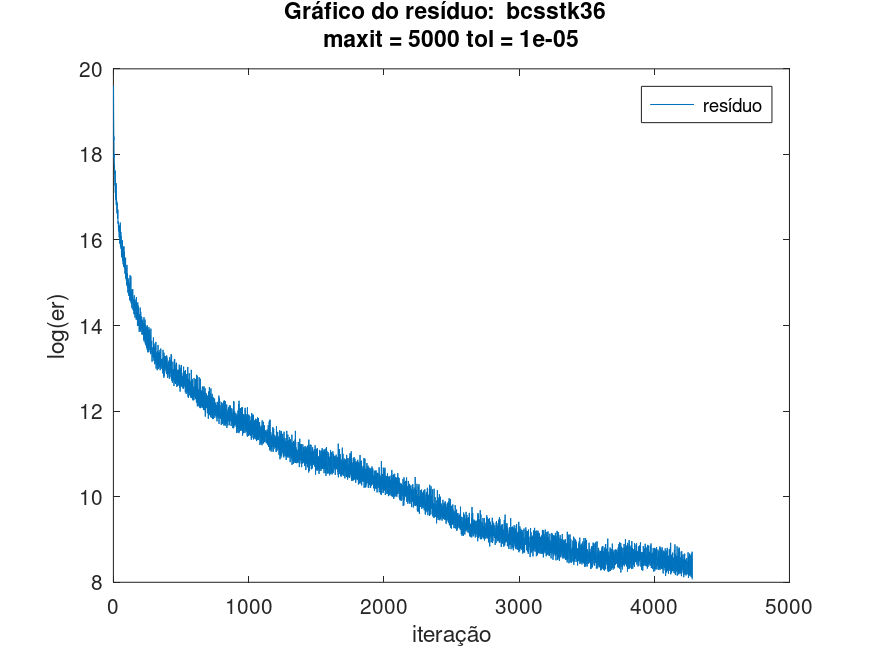
\includegraphics[width=\textwidth]{image/bcsstk36_5000_-6.png}
         \caption{Gráfico do Resíduo para maxit $= 5.000$ e tol $=10^{-6}$}
         \label{fig:bcsstk36-5-6}
    \end{subfigure}
    \quad
    \begin{subfigure}[t]{0.4\linewidth}
         \centering
         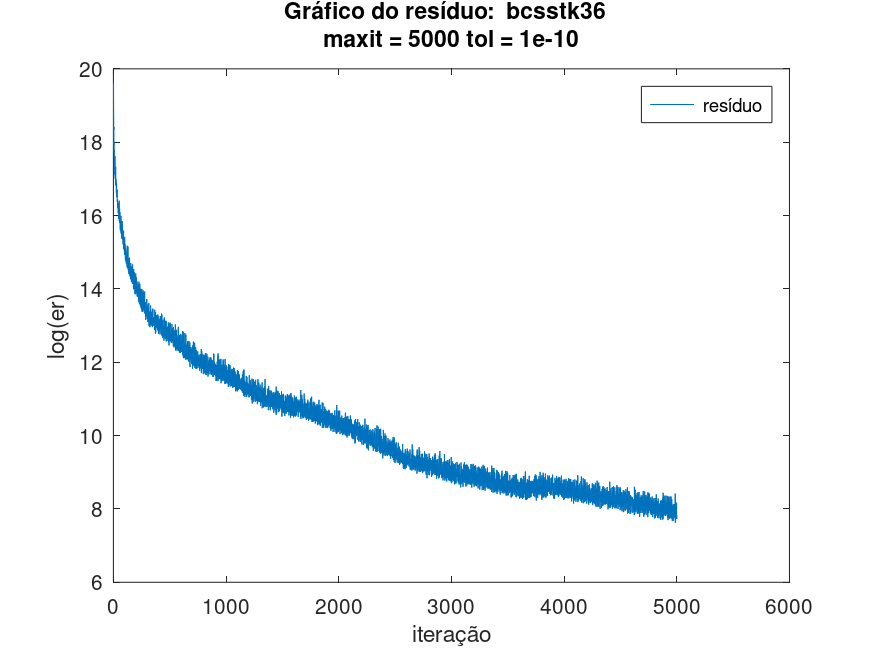
\includegraphics[width=\textwidth]{image/bcsstk36_5000_-11.png}
         \caption{Gráfico do Resíduo para maxit $= 5.000$ e tol $=10^{-11}$}
         \label{fig:bcsstk36-5-11}
    \end{subfigure}
    \par\bigskip
    \begin{subfigure}[t]{0.4\linewidth}
         \centering
         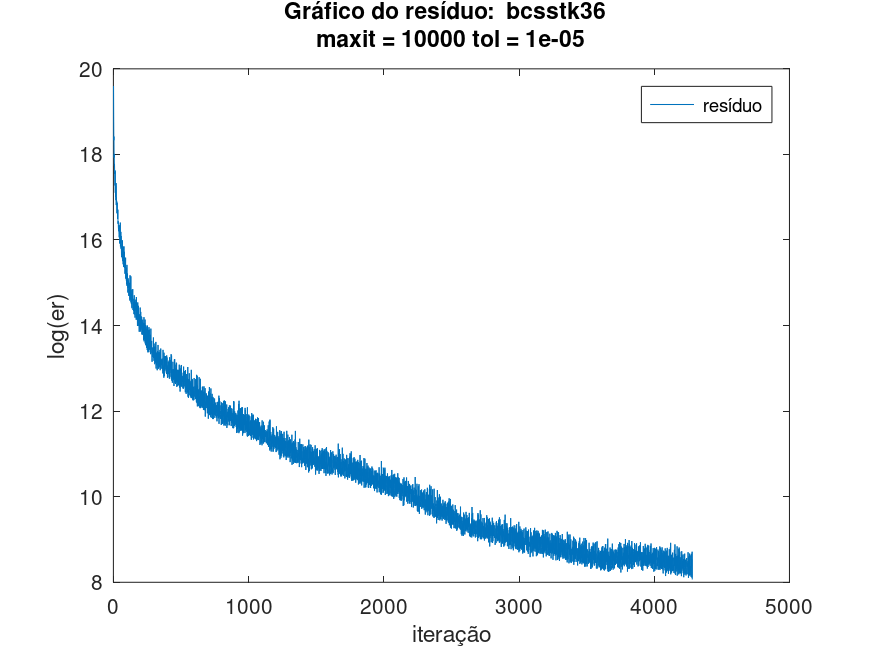
\includegraphics[width=\textwidth]{image/bcsstk36_10000_-6.png}
         \caption{Gráfico do Resíduo para maxit $= 10.000$ e tol $=10^{-6}$}
         \label{fig:bcsstk36-10-6}
    \end{subfigure}
    \quad
    \begin{subfigure}[t]{0.4\linewidth}
         \centering
         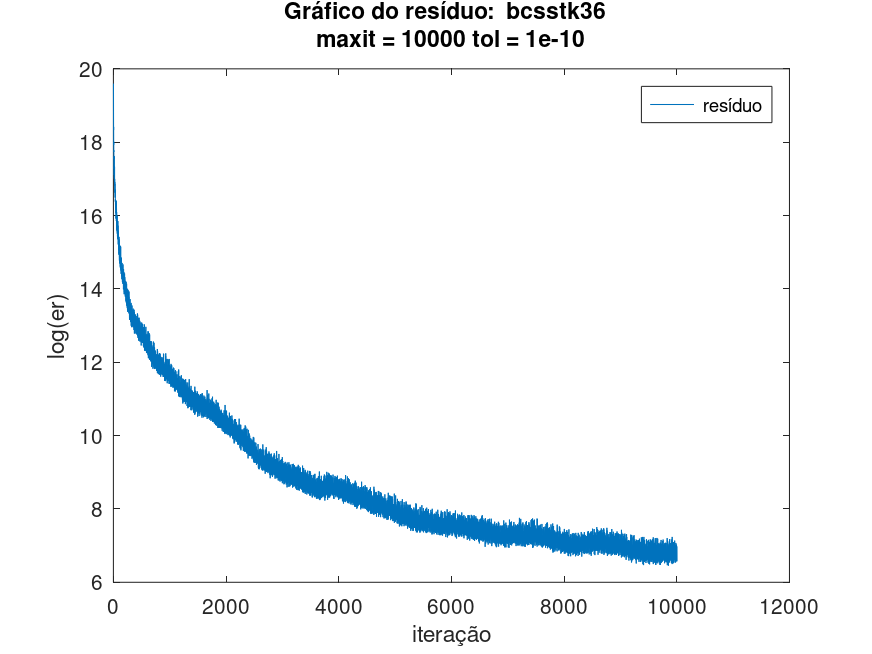
\includegraphics[width=\textwidth]{image/bcsstk36_10000_-11.png}
         \caption{Gráfico do Resíduo para maxit $= 10.000$ e tol $=10^{-11}$}
         \label{fig:bcsstk36-10-11}
    \end{subfigure}
    \caption{Gráficos dos resíduos para \textit{bcsstk36}.}
    \label{fig:bcsstk36}
\end{figure}
\begin{figure}[H]
    \centering
         \centering
         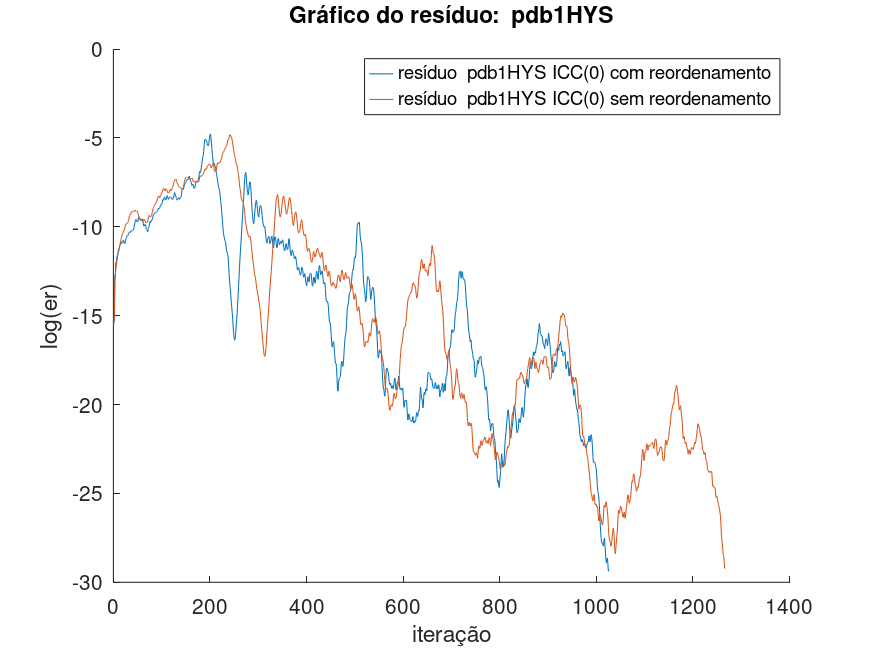
\includegraphics[width=.6\linewidth]{images/pdb1HYS.png}
         \caption{Gráfico do Resíduo da matriz \textit{pdb1HYS}}
         \label{fig:pdb-res}
\end{figure}

\begin{figure}[H]
    \centering
         \centering
         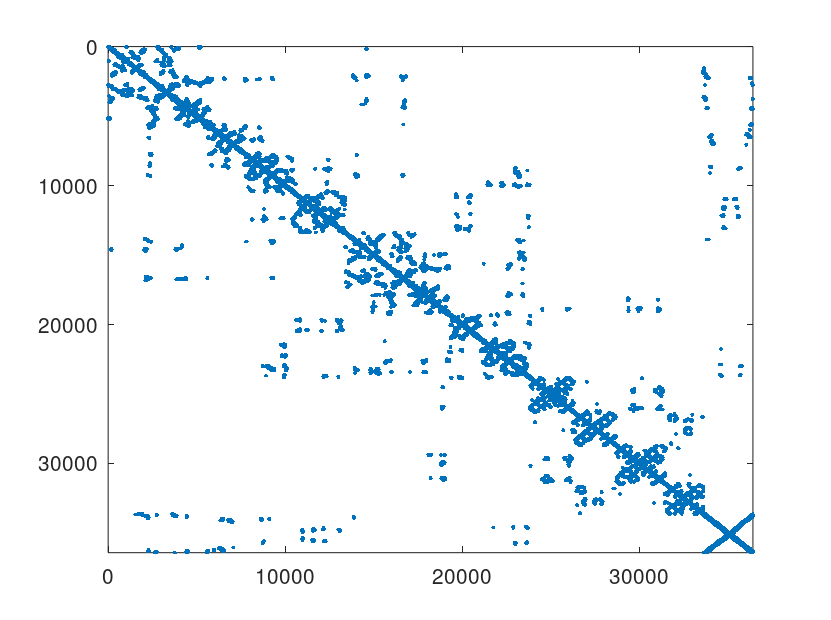
\includegraphics[width=.5\linewidth]{images/pdb1HYS_spyA.png}
         \caption{Spy de da matriz \textit{pdb1HYS}}
         \label{fig:pdb-spy-a}
\end{figure}

\begin{figure}[H]
    \centering
    \begin{subfigure}[t]{0.4\linewidth}
         \centering
         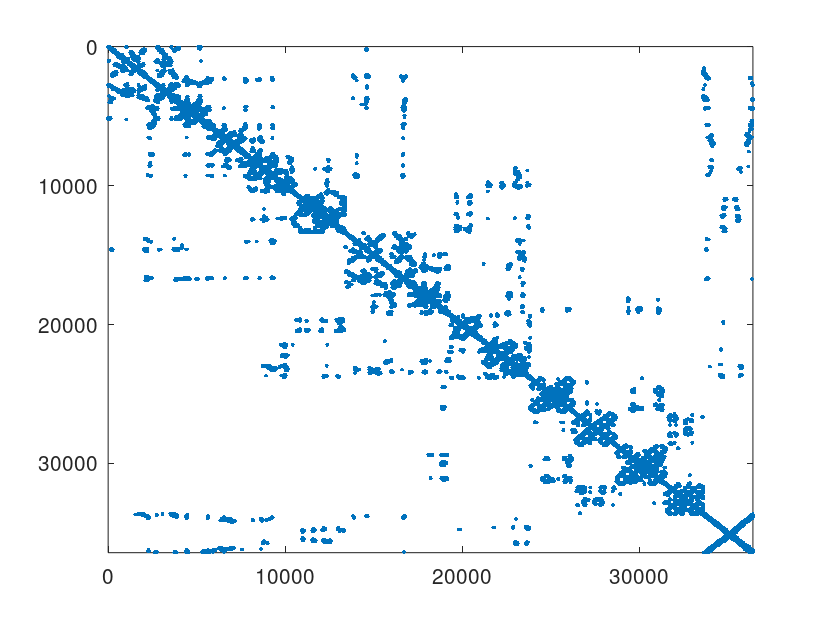
\includegraphics[width=\textwidth]{images/pdb1HYS_spyM_ICC(0)_sem.png}
         \caption{Spy após ICC(0) sem reordenamento}
         \label{fig:pdb-icc0-sem}
    \end{subfigure}
    \quad
    \begin{subfigure}[t]{0.4\linewidth}
         \centering
         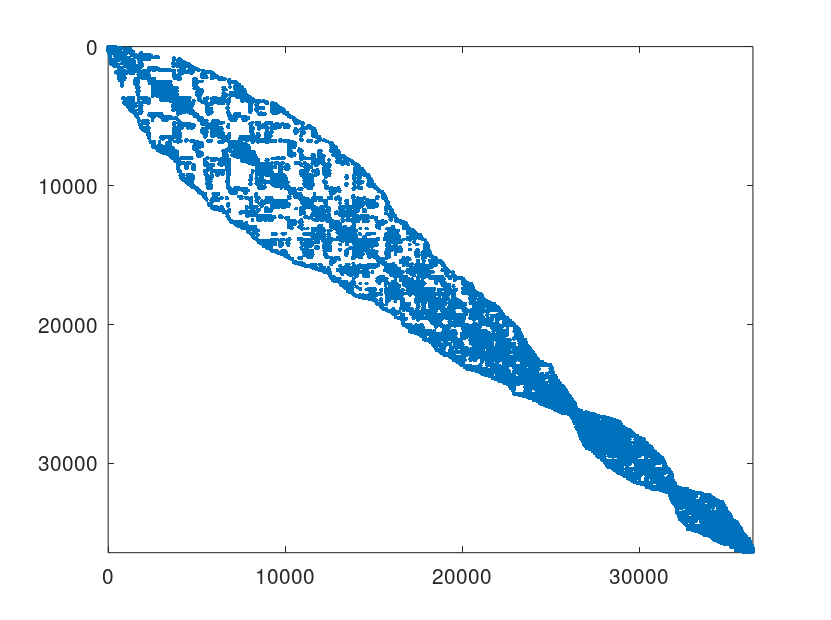
\includegraphics[width=\textwidth]{images/pdb1HYS_spyM_ICC(0)_com.png}
         \caption{Spy após ICC(0) com reordenamento}
         \label{fig:pdb-icc0-com}
    \end{subfigure}
    \label{fig:pdb}
\end{figure}
\begin{figure}[H]
    \centering
         \centering
         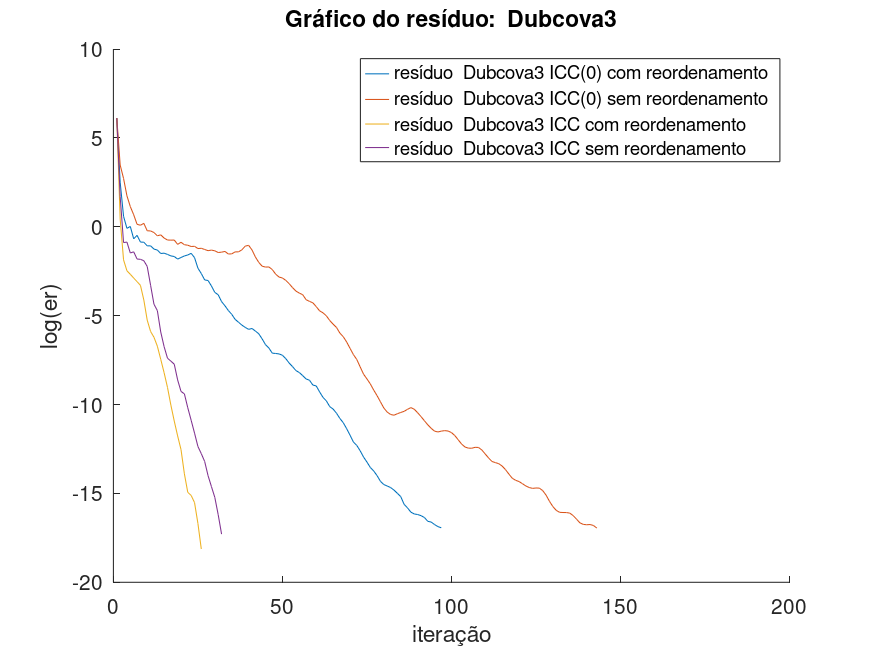
\includegraphics[width=.6\linewidth]{images/Dubcova3.png}
         \caption{Gráfico do Resíduo da matriz \textit{Dubcova3}}
         \label{fig:Dub-res}
\end{figure}



\section{Tabelas dos resultados observados}
\label{sec:tabelas}


\begin{table}[ht]
    \centering
    \begin{tabular}{|c|c|c|c|c|c|c|c|c|c|}
        \hline \rowcolor{Gray}
        \multicolumn{10}{|c|}{\bfseries Tabela do Método dos Gradientes Conjugados com tolerância $10^{-6}$ e máximo de iterações $5.000$ }\\
        \hline \rowcolor{Gray}  \multicolumn{5}{|c|}{} & \multicolumn{5}{|c|}{} \\
         [-1em]  \rowcolor{Gray}
         \multicolumn{5}{|c|}{\bfseries Informações da matriz } & \multicolumn{5}{|c|}{\bfseries Resultados do método }\\
         \hline \rowcolor{Gray} & & & & & & & & & \\
         [-1em]
         \rowcolor{Gray}
         \bfseries Nome & \bfseries n & \bfseries Elementos Não-nulos & \bfseries Diag. Dominante &
         k = cond(A) & flag & iterações &
         erro relativo &
         $\|x\|_\infty$  & tempo (s) \\
         \hline & & & & & & & & & \\
         [-1em] \bfseries mesh3em5 & 289 & 1377 & s & 4.965950e+00 & 0 & 11 & 3.750324e-06 & 1.000046e+00  & 0.0033319 s \\ & & & & & & & & & \\ [-1em] \hline \\
         [-1em] \bfseries plat362 & 362 & 5786 & n & 2.178231e+11 & 0 & 180 & 9.271656e-06 & 1.326850e+00  & 0.0303929 s \\ & & & & & & & & & \\ [-1em] \hline \\
         [-1em] \bfseries 662\_bus & 662 & 2474 & n & 7.941311e+05 & 0 & 385 & 8.556672e-06 & 1.000561e+00  & 0.0593071 s \\ & & & & & & & & & \\ [-1em] \hline \\
         [-1em] \bfseries s1rmq4m1 & 5489 & 262411 & n & 1.810479e+06 & 0 & 2442 & 9.021992e-06 & 1.039487e+00 & 2.60565 s \\ & & & & & & & & & \\ [-1em] \hline \\
         [-1em] \bfseries bcsstk36 & 23052 & 1143140 & n  & 7.433254e+11 & 0 & 4281 & 9.811595e-06 & 1.516600e+00 & 24.9607 s \\ & & & & & & & & & \\ [-1em] \hline \\
         [-1em] \bfseries pdb1HYS & 36417 & 4344765 & n & -- & 1 & 5001 & 3.854805e-05 & 1.000010e+00 & 77.0235 s \\ & & & & & & & & & \\ [-1em] \hline \\
         [-1em] \bfseries Dubcova3 & 146689 & 3636643 & n & -- & 0 & 134 & 9.039834e-06 & 1.000683e+00  & 2.75497 s \\ \hline
    \end{tabular}
    \caption{Tabela de resultados observados em resolução de matrizes pelo Método dos Gradientes Conjugados com tolerância $10^{-6}$ e máximo de iterações $5.000$.}
    \label{tab:resultados-5k-6}
\end{table}

\begin{table}[ht]
    \centering
    \begin{tabular}{|c|c|c|c|c|c|c|c|c|c|}
        \hline \rowcolor{Gray}
        \multicolumn{10}{|c|}{\bfseries Tabela do Método dos Gradientes Conjugados com tolerância $10^{-11}$ e máximo de iterações $5.000$ }\\
        \hline \rowcolor{Gray}  \multicolumn{5}{|c|}{} & \multicolumn{5}{|c|}{} \\
         [-1em]  \rowcolor{Gray}
         \multicolumn{5}{|c|}{\bfseries Informações da matriz } & \multicolumn{5}{|c|}{\bfseries Resultados do método }\\
         \hline \rowcolor{Gray} & & & & & & & & & \\
         [-1em]
         \rowcolor{Gray}
         \bfseries Nome & \bfseries n & \bfseries Elementos Não-nulos & \bfseries Diag. Dominante &
         k = cond(A) & flag & iterações &
         erro relativo &
         $\|x\|_\infty$  & tempo (s) \\
         \hline & & & & & & & & & \\
         [-1em] \bfseries mesh3em5 & 289 & 1377 & s & 4.965950e+00 & 0 & 20 & 6.495063e-12 & 1.000000e+00  & 0.00451517 s \\ & & & & & & & & & \\ [-1em] \hline \\
         [-1em] \bfseries plat362 & 362 & 5786 & n & 2.178231e+11 & 0 & 4090 & 9.928228e-11 & 1.027751e+00 & 0.560509 s \\ & & & & & & & & & \\ [-1em] \hline \\
         [-1em] \bfseries 662\_bus & 662 & 2474 & n & 7.941311e+05 & 0 & 678 & 8.627720e-11 & 1.000000e+00  & 0.0971811 s \\ & & & & & & & & & \\ [-1em] \hline \\
         [-1em] \bfseries s1rmq4m1 & 5489 & 262411 & n & 1.810479e+06 & 1 & 5001 & 3.787623e-09 & 1.000033e+00  & 5.06747 s \\ & & & & & & & & & \\ [-1em] \hline \\
         [-1em] \bfseries bcsstk36 & 23052 & 1143140 & n & 7.433254e+11 & 1 & 10001 & 6.295853e-06 & 1.694419e+00  & 28.219 s \\ & & & & & & & & & \\ [-1em] \hline \\
         [-1em] \bfseries pdb1HYS & 36417 & 4344765 & n & -- & 1 & 5001 & 3.854805e-05 & 1.000010e+00 & 73.3889 s \\ & & & & & & & & & \\ [-1em] \hline \\
         [-1em] \bfseries Dubcova3 & 146689 & 3636643 & n & -- & 0 & 215 & 9.438705e-11 & 1.000000e+00 & 4.33096 s \\ \hline 
    \end{tabular}
    \caption{Tabela de resultados observados em resolução de matrizes pelo Método dos Gradientes Conjugados com tolerância $10^{-11}$ e máximo de iterações $5.000$.}
    \label{tab:resultados-5k-11}
\end{table}

\begin{table}[ht]
    \centering
    \begin{tabular}{|c|c|c|c|c|c|c|c|c|c|}
        \hline \rowcolor{Gray}
        \multicolumn{10}{|c|}{\bfseries Tabela do Método dos Gradientes Conjugados com tolerância $10^{-6}$ e máximo de iterações $10.000$ }\\
        \hline \rowcolor{Gray}  \multicolumn{5}{|c|}{} & \multicolumn{5}{|c|}{} \\
         [-1em]  \rowcolor{Gray}
         \multicolumn{5}{|c|}{\bfseries Informações da matriz } & \multicolumn{5}{|c|}{\bfseries Resultados do método }\\
         \hline \rowcolor{Gray} & & & & & & & & & \\
         [-1em]
         \rowcolor{Gray}
         \bfseries Nome & \bfseries n & \bfseries Elementos Não-nulos & \bfseries Diag. Dominante &
         k = cond(A) & flag & iterações &
         erro relativo &
         $\|x\|_\infty$  & tempo (s) \\
         \hline & & & & & & & & & \\
         [-1em] \bfseries mesh3em5 & 289 & 1377 & s & 4.965950e+00 & 0 & 11 & 3.750324e-06 & 1.000046e+00 & 0.00355601 s \\ & & & & & & & & & \\ [-1em] \hline \\
         [-1em] \bfseries plat362 & 362 & 5786 & n &  2.178231e+11 & 0 & 180 & 9.271656e-06 & 1.326850e+00 & 0.025856 s \\ & & & & & & & & & \\ [-1em] \hline \\
         [-1em] \bfseries 662\_bus & 662 & 2474 & n &  7.941311e+05 & 0 & 385 & 8.556672e-06 & 1.000561e+00 & 0.066118 s \\ & & & & & & & & & \\ [-1em] \hline \\
         [-1em] \bfseries s1rmq4m1 & 5489 & 262411 & n & 1.810479e+06 & 0 & 2442 & 9.021992e-06 & 1.039487e+00 & 2.5727 s \\ & & & & & & & & & \\ [-1em] \hline \\
         [-1em] \bfseries bcsstk36 & 23052 & 1143140 & n & 7.433254e+11 & 0 & 4281 & 9.811595e-06 & 1.516600e+00 & 26.588 s \\ & & & & & & & & & \\ [-1em] \hline \\
         [-1em] \bfseries pdb1HYS & 36417 & 4344765 & n & -- & 0 & 6031 & 9.626156e-06 & 1.000001e+00 & 99.689 s \\ & & & & & & & & & \\ [-1em] \hline \\
         [-1em] \bfseries Dubcova3 & 146689 & 3636643 & n & -- & 0 & 134 & 9.039834e-06 & 1.000683e+00 & 2.70178 s \\ \hline
    \end{tabular}
    \caption{Tabela de resultados observados em resolução de matrizes pelo Método dos Gradientes Conjugados com tolerância $10^{-6}$ e máximo de iterações $10.000$.}
    \label{tab:resultados-10k-6}
\end{table}

\begin{table}[ht]
    \centering
    \begin{tabular}{|c|c|c|c|c|c|c|c|c| c|}
        \hline \rowcolor{Gray}
        \multicolumn{10}{|c|}{\bfseries Tabela do Método dos Gradientes Conjugados com tolerância $10^{-11}$ e máximo de iterações $10.000$ }\\
        \hline \rowcolor{Gray}  \multicolumn{5}{|c|}{} & \multicolumn{5}{|c|}{} \\
         [-1em]  \rowcolor{Gray}
         \multicolumn{5}{|c|}{\bfseries Informações da matriz } & \multicolumn{5}{|c|}{\bfseries Resultados do método }\\
         \hline \rowcolor{Gray} & & & & & & & & & \\
         [-1em]
         \rowcolor{Gray}
         \bfseries Nome & \bfseries n & \bfseries Elementos Não-nulos & \bfseries Diag. Dominante &
         k = cond(A) & flag & iterações &
         erro relativo &
         $\|x\|_\infty$  & tempo (s) \\
         \hline & & & & & & & & & \\
         [-1em] \bfseries mesh3em5 & 289 & 1377 & s & 4.965950e+00 & 0 & 20 & 6.495063e-12 & 1.000000e+00 & 0.00497293 s \\ & & & & & & & & & \\ [-1em] \hline \\
         [-1em] \bfseries plat362 & 362 & 5786 & n & 2.178231e+11 & 0 & 4090 & 9.928228e-11 & 1.027751e+00 & 0.554661 s \\ & & & & & & & & & \\ [-1em] \hline \\
         [-1em] \bfseries 662\_bus & 662 & 2474 & n & 7.941311e+05 & 0 & 678 & 8.627720e-11 & 1.000000e+00 & 0.100955 s \\ & & & & & & & & & \\ [-1em] \hline \\
         [-1em] \bfseries s1rmq4m1 & 5489 & 262411 & n  & 1.810479e+06 & 0 & 6417 & 9.360454e-11 & 1.000000e+00 & 7.74475 s \\ & & & & & & & & & \\ [-1em] \hline \\
         [-1em] \bfseries bcsstk36 & 23052 & 1143140 & n & 7.433254e+11 &  1 & 10001 & 1.955069e-06 & 1.492640e+00  & 58.3739 s \\ & & & & & & & & & \\ [-1em] \hline \\
         [-1em] \bfseries pdb1HYS & 36417 & 4344765 & n & -- & 3 & 6205 & 3.618273e-06 & 1.000001e+00 & 106.573 s \\ & & & & & & & & &\\ [-1em] \hline \\
         [-1em] \bfseries Dubcova3 & 146689 & 3636643 & n & -- & 0 & 215 & 9.438705e-11 & 1.000000e+00 & 4.30956 s \\  \hline
    \end{tabular}
    \caption{Tabela de resultados observados em resolução de matrizes pelo Método dos Gradientes Conjugados com tolerância $10^{-11}$ e máximo de iterações $10.000$.}
    \label{tab:resultados-10k-11}
\end{table}

\clearpage
\normalsetting

\end{document}
